\section{Sensitivity study}
This section performs a parametric sensitivity study of the reference tracking performance with respect to the number of past data points $\bar{N}$, the innovation noise variance $\sigma^2(e_k)$, and the window lengths $p=f$. As a measure of the reference tracking performance the root mean square of the reference tracking error, scaled by the root mean square of the reference signal, is used. To reflect purely the effect on performance during adaptive closed-loop operation, the considered means exclude control actions that rely in part on open-loop data (thus excluding the first $\bar{N}$ samples). Note that in general it is theoretically possible for \ac{DeePC} and \ac{CL-DeePC} to outperform the employed oracle because the oracle does (also) not account for noise.

\subsection{Number of past data samples: $\bar{N}$}
The effect of a varying number of past data samples $\bar{N}$ is shown in Fig.~\ref{fig:varying_Nbar}. Slight undulations of the displayed oracle performance are an artifact that is attributable to averaging over the last $1800-\bar{N}$ samples of a simulation to exclude control actions that are based on open-loop data. Using \ac{CL-DeePC} the reference tracking performance approaches the oracle's performance at a relatively low $\bar{N}$. For \ac{DeePC} the picture is different, with the median reference tracking performance remaining $26\%$ higher than its oracle counterpart at $\bar{N}=1039$. By comparison this value is only $4\%$ for \ac{CL-DeePC}.

Fig.~\ref{fig:varying_Nbar} demonstrates that \ac{CL-DeePC} is what we refer to as more `sample efficient' than \ac{DeePC}; in general \ac{CL-DeePC} is able to use fewer past data samples to obtain as good or better performance. The improved sample efficiency of \ac{CL-DeePC} is attributable to the fact that a shorter future prediction window length is implicitly used for identification by \ac{CL-DeePC} when compared to \ac{DeePC} ($f_\mathrm{ID}=1$ as opposed to $f_\mathrm{ID}=f$). This leaves more columns $N=\bar{N}-p-f_\mathrm{ID}+1$ to approximate the relevant correlation matrices that are used implicitly by both \ac{DeePC} and \ac{CL-DeePC} (consider, for instance, $Y_{i_p,1,f}\mathcal{Z}^\top=\hat{\Sigma}_{yz}$, $\hat{\Sigma}_{\psi z}$ from~\eqref{eq:Yfhat_1} and~\eqref{eq:Yfhat_2}). In addition, the discussed closed-loop identification issue entails that even if $\bar{N}$ (and therefore $N$) is large such that these correlation matrices are approximated well, \ac{DeePC} still performs worse than \ac{CL-DeePC}.
% ------------------------- Figure --------------------------
\begin{figure}[t!]
\begin{center}
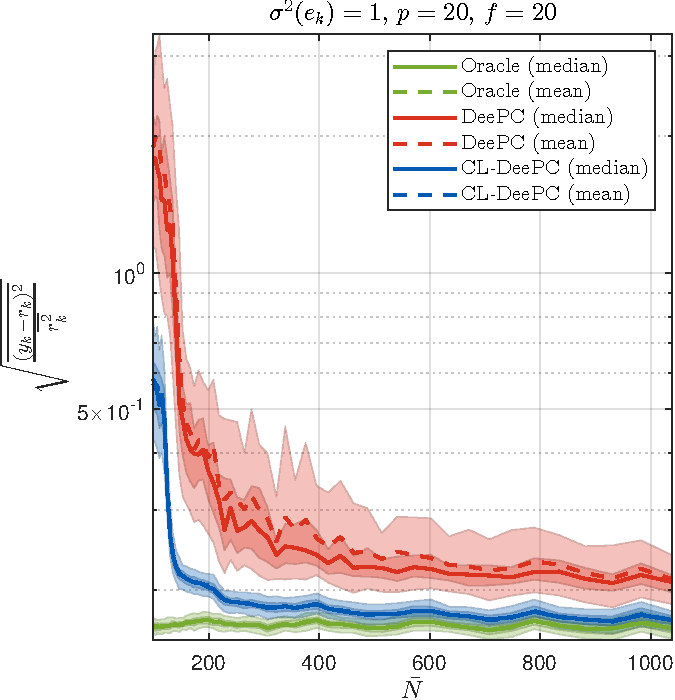
\includegraphics[width=\columnwidth]{results/figures/Varying_Nbar_99-1039-50_p_20_f_20_Re_1_Ru_1_Rdu_0_Q_100_R_0_dR_10.pdf}    % The printed column  
\caption{Effect of varying $\bar{N}$ on reference tracking performance. Shaded regions indicate the 1st, 3rd, 7th and 9th deciles of 120 simulations with different noise realizations.}  % width is 8.4 cm.
\label{fig:varying_Nbar}                                 % Size the figures 
\end{center}                                 % accordingly.
\end{figure}
% -----------------------------------------------------------

\subsection{Noise level: $\sigma^2(e_k)$}
The effect of the noise level, as quantified by a varying innovation noise variance $\sigma^2(e_k)$, is shown in Fig.~\ref{fig:varying_Re}. When there is little to no noise, 
% ------------------------- Figure --------------------------
\begin{figure}[b!]
\begin{center}
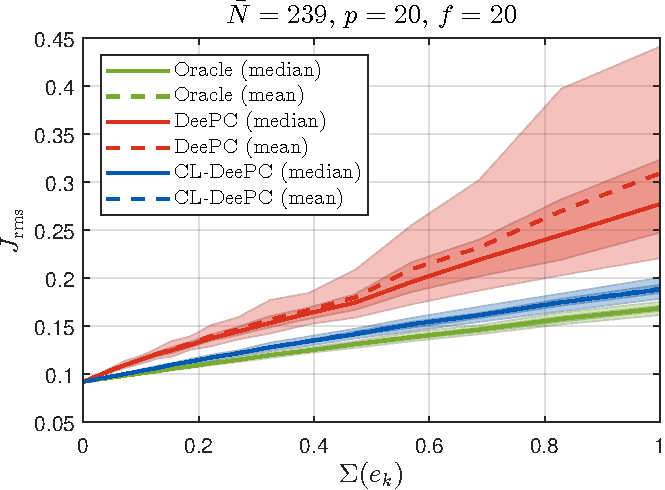
\includegraphics[width=\columnwidth]{results/figures/Varying_Re_0.0001-1-50_Nbar_239_p_20_f_20_Ru_1_Rdu_0_Q_100_R_0_dR_10.pdf}    % The printed column 
\caption{Effect of varying $\sigma^2(e_k)$ on reference tracking performance. Shaded regions indicate the 1st, 3rd, 7th and 9th deciles of 120 simulations with different noise realizations.}  % width is 8.4 cm.
\label{fig:varying_Re}                                 % Size the figures 
\end{center}                                 % accordingly.
\end{figure}
% -----------------------------------------------------------

\subsection{Past data window lengths: $p=f$}
1) period of 200 time samples
2) 
% ------------------------- Figure --------------------------
\begin{figure}[b!]
\begin{center}
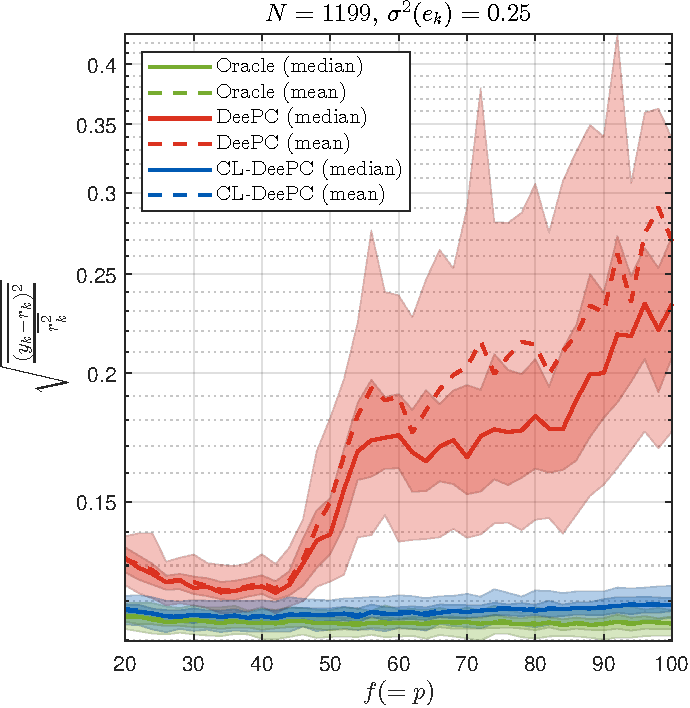
\includegraphics[width=\columnwidth]{results/figures/Varying_pf_20-100-41_Nbar_1199_Re_0.25_Ru_1_Rdu_0_Q_100_R_0_dR_10.pdf}    % The printed column 
\caption{Effect of varying $f=p$ on reference tracking performance. Shaded regions indicate the 1st, 3rd, 7th and 9th deciles of 120 simulations with different noise realizations.}  % width is 8.4 cm.
\label{fig:varying_Re}                                 % Size the figures 
\end{center}                                 % accordingly.
\end{figure}
% -----------------------------------------------------------
